\documentclass[BCOR0mm,fontsize=12pt,paper=a4,final,numbers=noenddot]{scrartcl}
%\usepackage[T1]{fontenc} % Für PDFLaTeX
\usepackage[utf8]{inputenc} 
\usepackage[hyphens]{url}
\usepackage[ngerman]{babel}
\usepackage{amsmath}
\usepackage{amssymb}
\usepackage[style=german]{csquotes}
\usepackage{setspace}
\usepackage{tocloft}
\usepackage[medium]{titlesec}
\usepackage{color}
\usepackage[inner=2.2cm,outer=2.2cm,top=2cm,bottom=2cm,includefoot,footskip=14mm]{geometry}
\usepackage{scrpage2}
\usepackage[final]{microtype}
\usepackage{soul}
\usepackage{blindtext}
\usepackage{paralist}
\usepackage{upgreek}
\usepackage{lscape}
\usepackage{enumitem} 
\usepackage{longtable}
\usepackage{tabu}
\usepackage[]{listings}
\usepackage{graphicx}
\usepackage{tikz-er2}
\usepackage{verbatim}
\usepackage{ulem}


% Einstellungen für Listings
\definecolor{grey}{rgb}{0.4, 0.45, 0.41}
\lstset{language=Java,
                basicstyle=\ttfamily\footnotesize,
                keywordstyle=\color{blue}\ttfamily,
                stringstyle=\color{red}\ttfamily,
                commentstyle=\color{grey}\ttfamily,
                morecomment=[l][\color{grey}]{\#},
                showstringspaces=false}

\pagestyle{plain}

% Auslassungszeichen

\renewcommand{\dots}{[\ldots]}

\begin{document}
\makeatletter         

% Kapitelüberschriften
\renewcommand*{\thesubsection}{\@arabic\c@subsection.}
\titleformat{\section}[hang]{\sffamily\bfseries\LARGE\centering}{\thesection}{5pt}{}
\titleformat{\subsection}[hang]{\sffamily\bfseries\Large}{\thesubsection}{5pt}{}
%\renewcommand*{\raggedsection}{\centering}


\makeatother


\setlength{\baselineskip}{11pt}

\noindent{}\begin{footnotesize}Freie Universität Berlin\\
Institut für Informatik\\
Datenbanksysteme\\
Sommersemester 2017\\
Bearbeiter: Felix Binder, Nicolas Höcker, Armin Weber\\
\end{footnotesize}

\setlength{\baselineskip}{12pt}

\bigskip

\section*{Projektdokumentation}

\onehalfspacing

\subsection{Projektziel}

Ziel des Projekts ist es, eine "`Projekt"=Web"=Anwendung"' zu erstellen, mit deren Hilfe der Datensatz "`american"=election"=tweets"' analysiert werden kann. Analysieren heißt hier, dass die Anwendung in der Lage sein soll, das Beziehungsgeflecht zwischen den in den Tweets verwendeten Hashtags grafisch darzustellen und mittels benutzerdefinierter Anfragen weitere Informationen aus den Daten zu gewinnen. So soll es unter anderem möglich sein, die am meisten verwendeten Hashtags zu identifizieren, Aussagen über deren paarweise gemeinsames Auftreten zu treffen und die Wichtigkeit einzelner Tweets zu bewerten. Auch Auswertungen dessen, wie sich die einzelnen Punkte über die Zeit hinweg verändert haben, sollen möglich sein.

% (Anmerkung für uns: Das Projekt hat also zwei Seiten: 1. Das ganze technisch umsetzen. 2. Nebenbei ein Maß für zunächst rein semantische Sachverhalte wie "`Wichtigkeit"' finden, so dass sich Daten aus dem Datensatz gewichten lassen.)

\subsection{Team}

\paragraph*{Felix Binder:} Studiert Philosophie und Informatik (60 LP) gegen Ende seines Bachelorstudiums.

\paragraph*{Nicolas Höcker:} Studiert Informatik im 4. Bachelorsemester.

\paragraph*{Armin Weber:} Studiert Informatik im vierten Semester.


\subsection{Explorative Datenanalyse}

Der Datensatz besteht aus 6126 Tweets, die zwischen dem 5.~Januar 2016 und dem 28.~September 2016 über die Twitter"=Konten \textit{realDonaldTrump} und \textit{HillaryClinton} abgesetzt, d.\,\,h. von diesen selbst verfasst oder retweetet wurden. Das jeweilige Twitter"=Konto findet sich dabei in der ersten Spalte des Datensatzes ("`handle"'); die Information, ob es sich um einen Retweet handelt, in der dritten Spalte ("`is\_retweet"'), in der vierten bei Retweets der ursprüngliche Autor ("`original\_author"'). Der Text selbst -- und mit ihm alle Hashtags -- befindet sich in der zweiten Spalte.

Darüber hinaus enthält der Datensatz Informationen darüber, ob der Text ein Zitat ist und also auf eine andere Quelle verweist (siebte Spalte, "`is\_quote\_status"', mit der Quelle in der neunten Spalte, "`source\_url"') sowie dabei evtl. abgekürzt wurde (zehnte Spalte, "`truncated"'), ob der jeweilige Tweet eine Antwort auf einen anderen Tweet darstellt (sechste Spalte, "`in\_reply\_to\_screen\_name"'), wie oft er retweetet wurde und wie oft favorisiert (Spalten 7 und 8).

Dem ersten Augenschein nach sind für uns von Bedeutung:

\begin{enumerate}[label=\alph*),nosep]
 \item die Spalte Text, um daraus die Hashtags zu extrahieren;
 \item die Spalte mit dem Datum und der Uhrzeit, um das unterschiedlich starke Vorkommen von Hashtags zu verschiedenen Zeitpunkten nachvollziehen zu können;
 \item die Spalten zu Retweets und Favorisierungen, weil sie Indikatoren für die Wichtigkeit von Tweets sind.
\end{enumerate}

Die weiteren Spalten scheinen auf den ersten Blick für unsere Zwecke vernachlässigbar zu sein.


\clearpage

\subsection{ER"=Modellierung}

Das ER"=Modell für das Projekt sieht wie folgt aus:

\bigskip

\usetikzlibrary{positioning}
\usetikzlibrary{shadows}

\begin{footnotesize}

\begin{tikzpicture}[node distance=4em]
 \node[entity] (tweet) {Tweet};
    \node[attribute] (handle) [above=9em of tweet] {handle} edge (tweet);
    \node[attribute] (id) [below left=2cm of tweet] {\key{ID}} edge (tweet);
    \node[attribute] (text) [above= 6em of id] {text} edge (tweet);
    \node[attribute] (time) [above=2em of id] {time} edge (tweet);
    \node[attribute] (is_q) [above= 10em of id,align=center] {is\_quote\_\\status} edge (tweet);
    \node[attribute] (favorite_count) [above=16em of id] {favorite\_count} edge (tweet.120);
    \node[derived attribute] (imp) [right=of handle] {Wichtigkeit} edge (tweet);
    \node[attribute] (retweet_count) [below=2em of id] {retweet\_count} edge (tweet);
    \node[attribute] (is_r) [below=8em of tweet] {is\_retweet} edge (tweet);
 
%  \node[relationship] (schreibt) [above=2cm of tweet] {schreibt} edge [total] node[auto,swap]{N} (tweet);
%  
%  \node[entity] (autor) [above=2cm of schreibt] {Autor} edge node[auto,swap]{1} (schreibt);
%     \node[attribute] (hanlde) [left=of autor] {\key{handle}} edge (autor);
%     
%  \node[relationship] (retweetet) [right=0.4cm of schreibt] {retweetet} edge node[auto,swap]{1} (autor);
%     \node[attribute] (orig) [above right=of retweetet] {original\_author} edge (retweetet);
%     \draw[link]  (tweet)  -/ node[left,swap]{N} (retweetet);
%     
 \node[relationship] (enth) [right=2cm of tweet] {enthält} edge node[auto,swap]{N} (tweet);
    \node[attribute] (oft) [above right=of enth] {wie\_oft} edge (enth);
 \node[entity] (hash) [right=2cm of enth] {Hashtag} edge [total] node[auto,swap]{M} (enth);
    \node[attribute] (name) [above=of hash] {\key{Name}} edge (hash);
    \node[attribute] (anz) [above right=0.7cm of hash, align=center] {Anzahl\_\\global} edge (hash);
 
 \node[relationship] (bilden) [below=1.4cm of hash] {bilden} edge node[auto,swap]{2} (hash);
 
 \node[relationship] (ent) [below right=3cm of tweet] {enthält} edge node[auto,swap]{N} (tweet);
    \node[attribute] (w_oft) [below=of ent] {wie\_oft} edge (ent);
    
 \node[entity] (hash_p) [below=5cm of hash,align=center] {Hashtag-\\Paare} edge [total] node[auto,swap]{M} (ent);
    \node[attribute] (anzahl) [below= of hash_p] {Anzahl\_global} edge (hash_p);
    \node[attribute] (hp_id) [below right=1cm of hash_p] {\key{ID}} edge (hash_p);
    
 \draw[link] [total] (bilden)  -/ node[right,swap]{M} (hash_p);
    
\end{tikzpicture}

\end{footnotesize}

\noindent{}Dieses Modell enthält augenblicklich noch mehr Informationen, als für die Beantwortung der in Abschnitt 1 genannten Fragen nötig wäre. So wäre es eigentlich unnötig abzuspeichern, ob ein Tweet ein Retweet oder ein Zitat ist. Allerdings wollen wir die Option offenhalten, in der fertigen Anwendung zu untersuchen, ob es signifikante Unterschiede hinsichtlich der Wichtigkeit der Tweets der verschiedenen Arten gibt. Da wir solche Unterschiede nicht ausschließen können, scheint uns das Weglassen solcher Informationen zu diesem frühen Zeitpunkt nicht angeraten.

Davon abgesehen war unser Anliegen, immer die naheliegenden Entscheidungen zu treffen: etwa Hashtag"=Paare aus Hashtags zusammenzusetzen und in den Relationen alle Informationen zu speichern, die später abrufbar sein sollen, etwa wie oft Hashtags in einzelnen Tweets vorkommen. Dort, wo es sinnvoll erschien, haben wir als Schlüssel außerdem eigenständige IDs ergänzt, um keine zu komplexen Schlüssel verwenden zu müssen (wie es bei den Tweets sonst etwa der Fall wäre).

Außerdem haben wir uns nach einigem Hin und Her dazu entschlossen, den Autor eines Tweets als Attribut handle in das Modell zu integrieren statt als eigene Entität. Hätten wir ihn als eigene Entität modelliert, die zu Tweets in den Relationen "`schreibt"' und "`retweetet"' steht, so hätten wir eine Tabelle mit nur einem einzigen Attribut (eben "`handle"'), wohingegen alle Attribute der Relationen zu "`Tweet"' gezogen hätten werden können, da es sich um 1:N"=Relationen gehandelt hätte. Damit hätte man für Abfragen nach dem Autor eines Tweets eigens mehrere Tabellen mittels JOIN verbinden müssen, was gerade bei Abfragen von den Hashtags her reichlich komplex geworden wäre, ohne dass das Ausgliedern des Autors als Entität irgendeinen Vorteil zu versprechen schien.


\subsection{Relationales Modell}

\noindent\textsc{Tweet}(\uline{ID}, handle, text, time, is\_retweet, is\_quote\_status, retweet\_count, favorite\_count)

\noindent\textsc{Hashtag}(\uline{Name}, Anzahl\_global)

\noindent\textsc{T\_enth\_H}(\uline{\dashuline{Tweet\_ID}, \dashuline{H\_Name}}, wie\_oft)

\noindent\textsc{Hashtag\_Paare}(\uline{ID}, Anzahl\_global)

\noindent\textsc{Hashtags\_bilden\_HP}(\uline{\dashuline{Hash\_Name}, \dashuline{HP\_ID}})

\noindent\textsc{T\_enth\_HP}(\uline{\dashuline{Tweet\_ID}, \dashuline{Hashpaar\_ID}}, wie\_oft)

\subsection{Datenbank}
Wir haben eine Datenbank \textit{Election} erstellt.

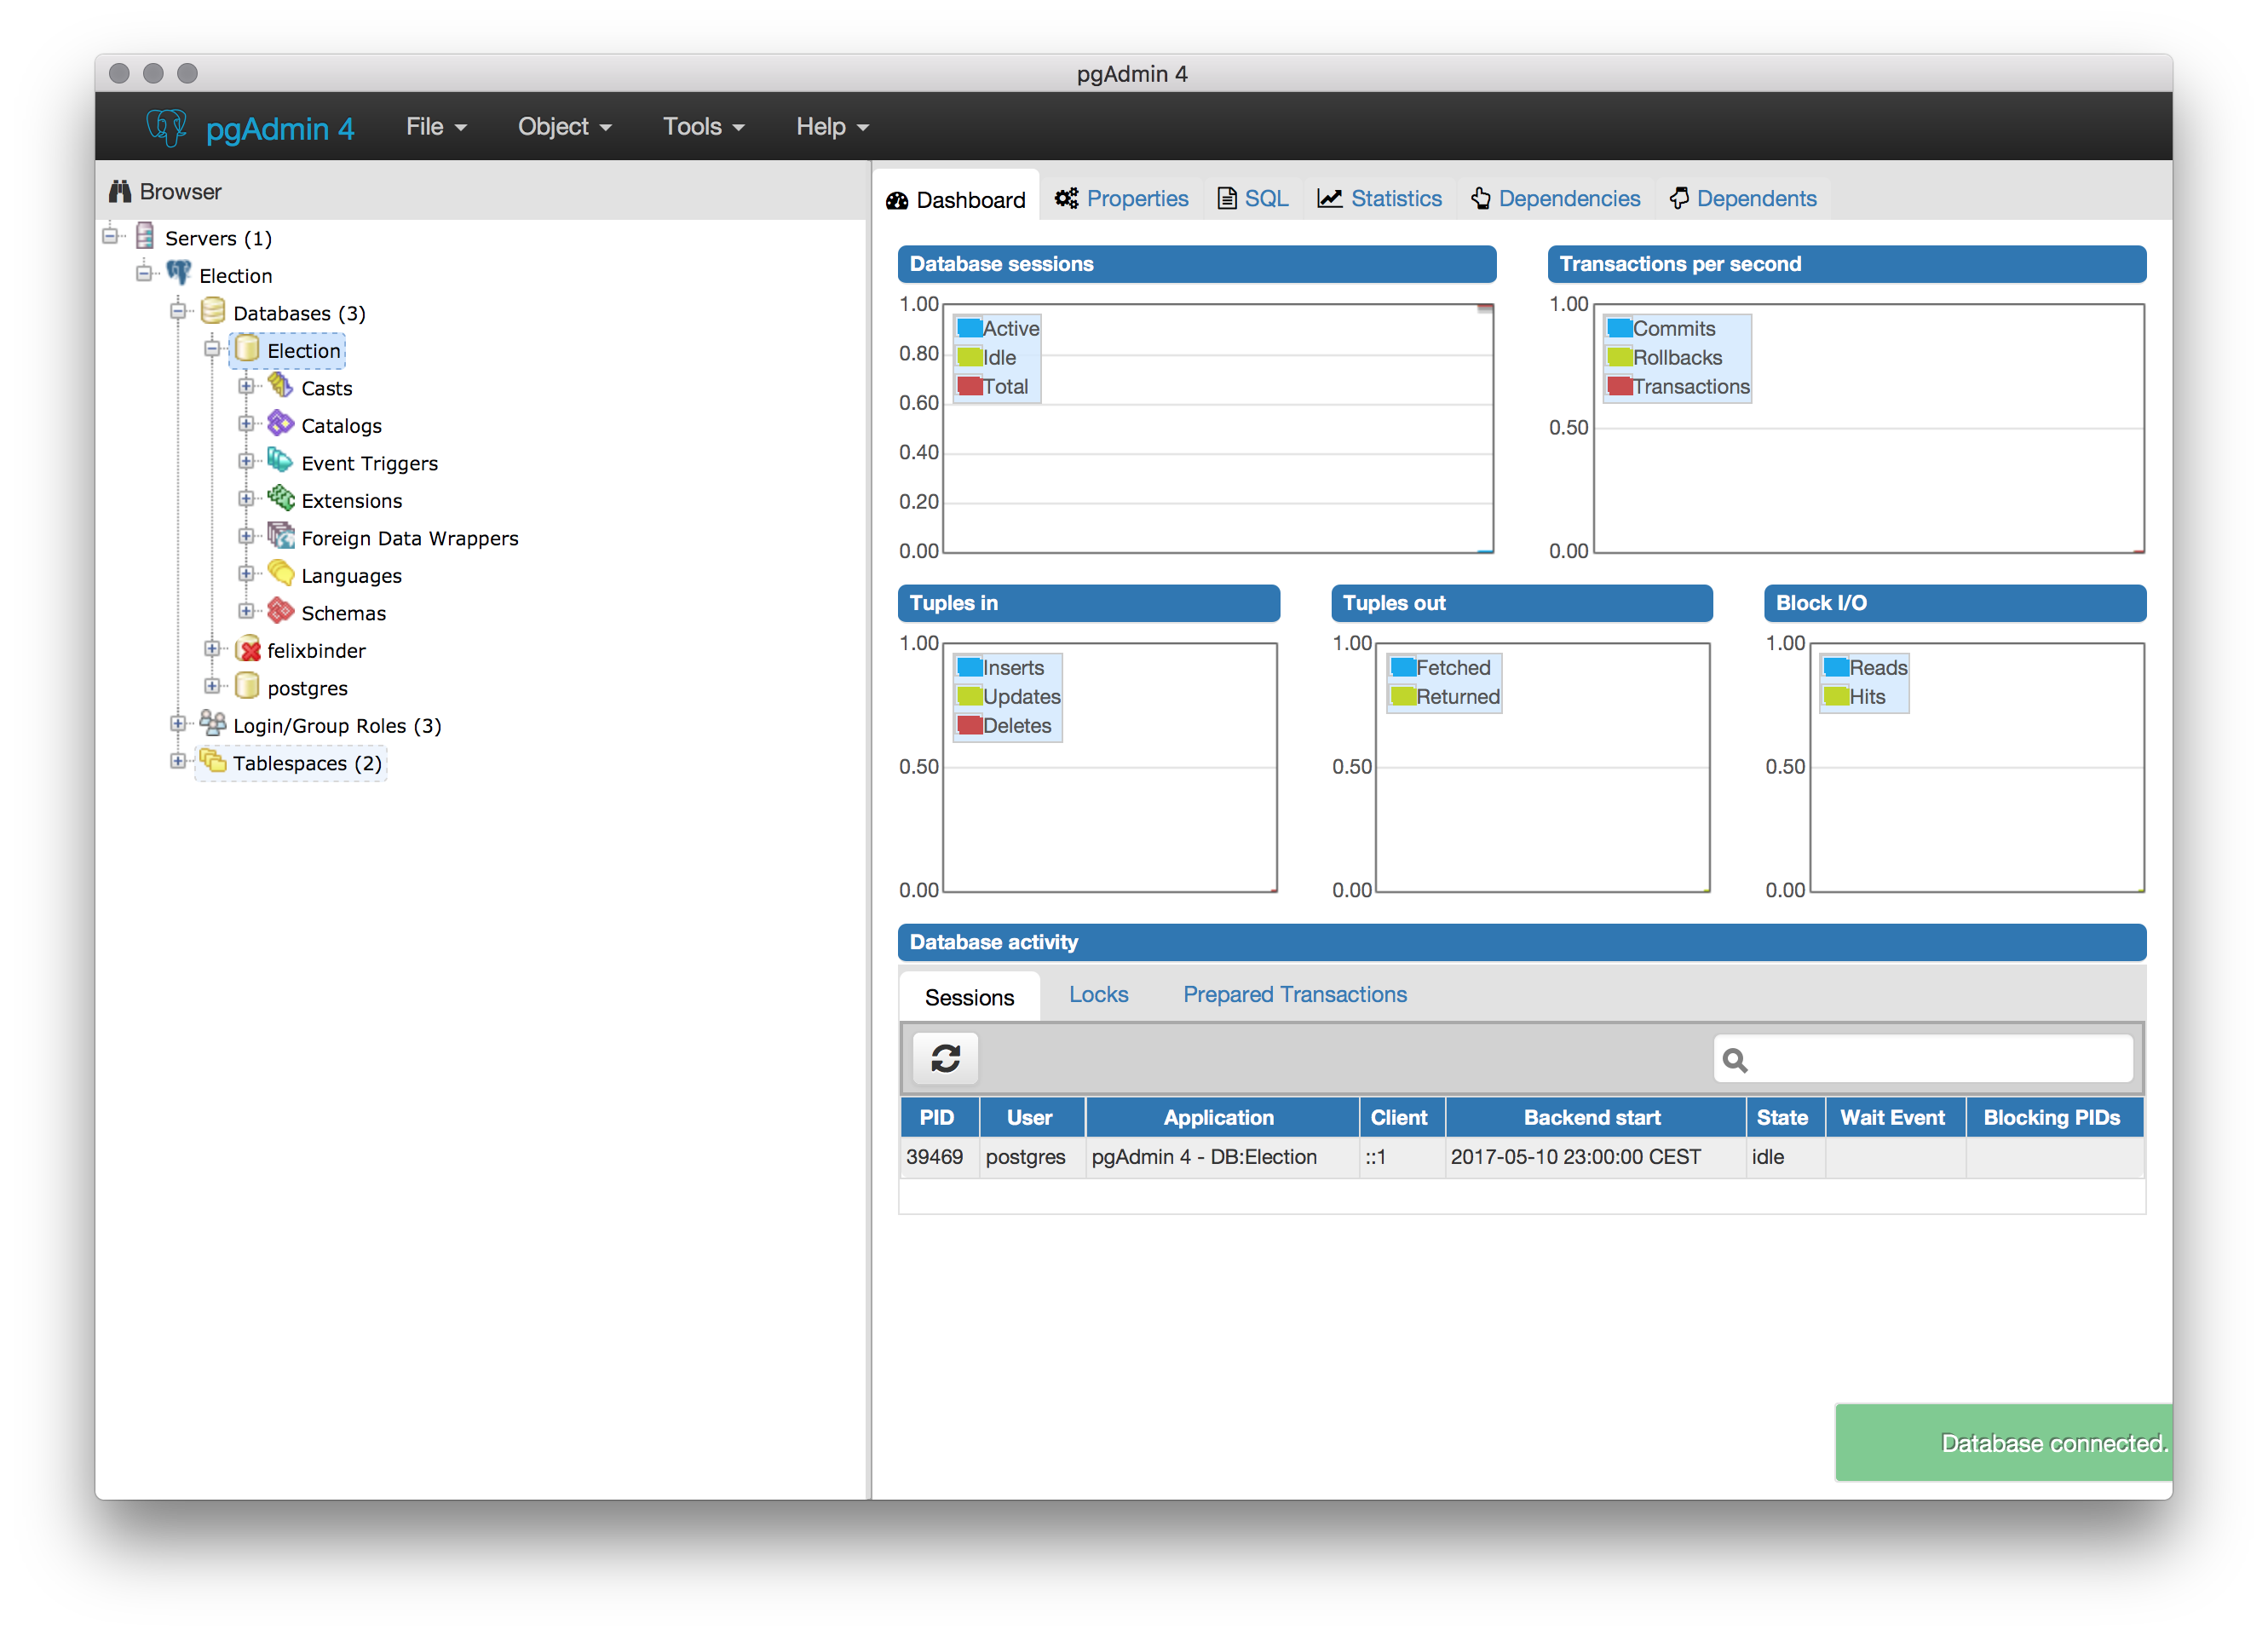
\includegraphics[width=0.95\textwidth]{datenbank_beweis.png}

Der Code dafür war:
\begin{verbatim}
	CREATE DATABASE "Election"
	    WITH 
	    OWNER = postgres
	    ENCODING = 'UTF8'
	    CONNECTION LIMIT = -1;
\end{verbatim}

\end{document}
